%\documentclass{beamer}
%Для защит онлайн лучше использовать разрешение 16x9
\documentclass[aspectratio=169]{beamer}

% !TeX spellcheck = ru_RU
% !TEX root = vkr.tex
% Опциональные добавления используемых пакетов. Вполне может быть, что они вам не понадобятся, но в шаблоне приведены примеры их использования.
\usepackage{tikz} % Мощный пакет для создание рисунков, однако может очень сильно замедлять компиляцию
\usetikzlibrary{decorations.pathreplacing,calc,shapes,positioning,tikzmark}

% Библиотека для TikZ, которая генерирует отдельные файлы для каждого рисунка
% Позволяет ускорить компиляцию, однако имеет свои ограничения
% Например, ломает пример выделения кода в листинге из шаблона
% \usetikzlibrary{external}
% \tikzexternalize[prefix=figures/]

\newcounter{tmkcount}

\tikzset{
  use tikzmark/.style={
    remember picture,
    overlay,
    execute at end picture={
      \stepcounter{tmkcount}
    },
  },
  tikzmark suffix={-\thetmkcount}
}

\usepackage{booktabs} % Пакет для верстки "более книжных" таблиц, вполне годится для оформления результатов
% В шаблоне есть команда \multirowcell, которой нужен этот пакет.
\usepackage{multirow}
\usepackage{siunitx} % для таблиц с единицами измерений

\newcommand{\cd}[1]{\texttt{#1}}
\newcommand{\inbr}[1]{\left<#1\right>}

% Для названий стоит использовать \textsc{}
\newcommand{\OCaml}{\textsc{OCaml}}
\newcommand{\miniKanren}{\textsc{miniKanren}}
\newcommand{\BibTeX}{\textsc{BibTeX}}
\newcommand{\vsharp}{\textsc{V$\sharp$}}
\newcommand{\fsharp}{\textsc{F$\sharp$}}
\newcommand{\csharp}{\textsc{C$\sharp$}}
\newcommand{\GitHub}{\textsc{GitHub}}
\newcommand{\SMT}{\textsc{SMT}}

\newcolumntype{L}[1]{>{\raggedright\let\newline\\\arraybackslash\hspace{0pt}}m{#1}}
%\newcolumntype{C}[1]{>{\centering\let\newline\\\arraybackslash\hspace{0pt}}m{#1}}
\newcolumntype{R}[1]{>{\raggedleft\let\newline\\\arraybackslash\hspace{0pt}}m{#1}}

\usepackage{xcolor}

%  Команды и пакеты, не используемые в шаблоне, которые тем не менее могут быть полезными.

% \newcolumntype{Y}{>{\centering\arraybackslash}X}

% \usepackage{mathrsfs}

\lstdefinestyle{fsharp}{
  basicstyle=\small\ttfamily,
  keywordstyle=\color{blue},
  commentstyle=\color{lightblue},
  stringstyle=\color{red},
  numbers=left,
  numberstyle=\tiny\color{gray},
  stepnumber=1,
  numbersep=10pt,
  backgroundcolor=\color{white},
  showspaces=false,
  showstringspaces=false,
  showtabs=false,
  tabsize=2,
  breaklines=true,
  breakatwhitespace=false,
  morekeywords={async, let, rec, if, then, else, do, yield, return, use, match, with, function}
  literate={->}{{$\to$}}3 {==}{{$\equiv$}}1 {=/=}{{$\not\equiv$}}1 {|>}{{$\triangleright$}}3 {\\/}{{$\vee$}}2 {/\\}{{$\wedge$}}2 {>=}{{$\ge$}}1 {<=}{{$\le$}}
}


% То, что в квадратных скобках, отображается внизу по центру каждого слайда. 
\title[GPU Image Processing]{Реализация библиотеки по обработке изображений с использованием GPU для платформы .NET}

% То, что в квадратных скобках, отображается в левом нижнем углу. 
\institute[СПбГУ]{}

% То, что в квадратных скобках, отображается в левом нижнем углу.
\author[Савельева Полина]{Савельева Полина Андреевна, группа 22.Б07-мм}
 
\begin{document}
{
\setbeamertemplate{footline}{}
% Лого университета или организации, отображается в шапке титульного листа
\begin{frame}
  
\includegraphics[width=1.4cm]{pictures/SPbGU_Logo.png}
\vspace{-35pt}
\hspace{-10pt}
\begin{center}
   \begin{tabular}{c}
        \scriptsize{Санкт-Петербургский государственный университет} \\
        %\scriptsize{Кафедра системного программирования}
    \end{tabular}
\titlepage
\end{center}

\btVFill

{\scriptsize
  % У научного руководителя должна быть указана научная степень
   \textbf{Научный руководитель:} к.~ф.-м.~н. С.~В.~Григорьев, доцент кафедры информатики \\
  % Консультанта может и не быть. Должна быть указана должность или ученая степень
   %\textbf{Консультант:}  П.П. Петров, программист ЗАО \enquote{Компания с ну очень-очень-очень длинным названием}\\
  % Для курсовой не обязателен. Должна быть указана должность или ученая степень
   %\textbf{Рецензент:} д.т.н., проф. И.И. Иванов, исполнительный директор ООО \enquote{Рога и копыта}  
 }
\begin{center}
  \vspace{5pt}
  \scriptsize{Санкт-Петербург\\
                 2023}
  \end{center}

\end{frame}
}

\begin{frame}[fragile]  
  \frametitle{Введение}
  \begin{itemize}
    \item Использование GPU значительно ускоряет обработку изображений и снижает нагрузку на CPU
    \item Доступность графических процессоров позволяет применять их в сферах, где требуется обрабатывать большое количество данных (компьютерное зрение, медицина, графика и дизайн)
    \item Идея --- предоставить .NET разработчикам инструмент, позволяющий эффективно использовать возможности GPU при работе с изображениями
  \end{itemize}
\end{frame}
            
\begin{frame}  
  \frametitle{Существующие решения}
  
  \begin{itemize}
    \item
    \item Указать их преимущества и недостатки (критика существующих решений/подходов)  
     Возможно, предметная область сложна и потребуется больше одного слайда, но затягивать введение не стоит. Постарайтесь уложиться в 1--2 слайда
  \end{itemize}
  \begin{itemize}
    \item Выводы
    \begin{itemize}
      \item Подвести итог
      \item Указать недостатки существующих подходов, на борьбу с которыми 
направленна данная работа
      \item Чётко сформулировать существующую проблему, которая будет решаться в данной работе
  \end{itemize}
  \end{itemize}
    
\end{frame}

% Обязательный слайд: четкая формулировка цели данной работы и постановка задачи
% Описание выносимых на защиту результатов, процесса или особенностей их достижения и т.д.
\begin{frame}
  \frametitle{Постановка задачи}
  \textbf{Целью} работы является реализация библиотеки по обработке изображений с использованием GPU %озвученной выше 
  
  \textbf{Задачи}:
  \begin{itemize}
    \item Добавить следующие возможности:
    \begin{itemize}
        \item Сохранение в различных форматах (исходное изображение в png сохранить в jpeg)
        \item Скос (skew)
        \item Изменение размера (reseize)
        \item Обрезка (crop)
        \item Добавление водяного знака (watermark)
    \end{itemize}
    \item Сравнить производительности текущей реализации и аналогов 
    \item Оформить и опубликовать GitHub пакет
  \end{itemize}
\end{frame}
            
%Идеально, если есть по одному слайду на каждую поставленную задачу            
\begin{frame}
  \frametitle{Языки .NET}
  \begin{minipage}[m]{0.6\linewidth}
        \begin{figure}
            \centering
            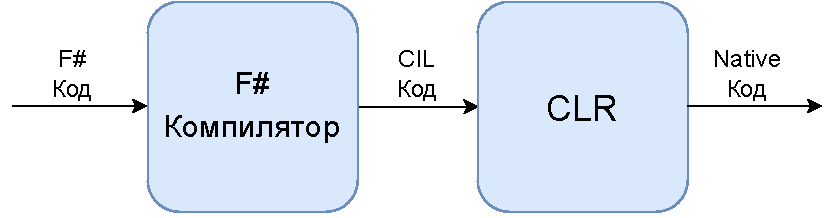
\includegraphics[width=8.0cm]{pictures/CIL.pdf}
            \caption{Трансляция языков .NET}
            \label{fig:cil}
        \end{figure}
    \end{minipage}\hfill
    \begin{minipage}[m]{0.4\linewidth}
        Выбор .NET языков при написании библиотеки может иметь несколько причин:
    \begin{itemize}
        \item Богатая экосистема .NET
        \item Переносимость
        \item Высокая производительность
    \end{itemize}
    \end{minipage}
\end{frame}

\begin{frame}
  \frametitle{GPU-вычисления}
  \begin{minipage}[m]{0.6\linewidth}
        \begin{figure}
            \centering
            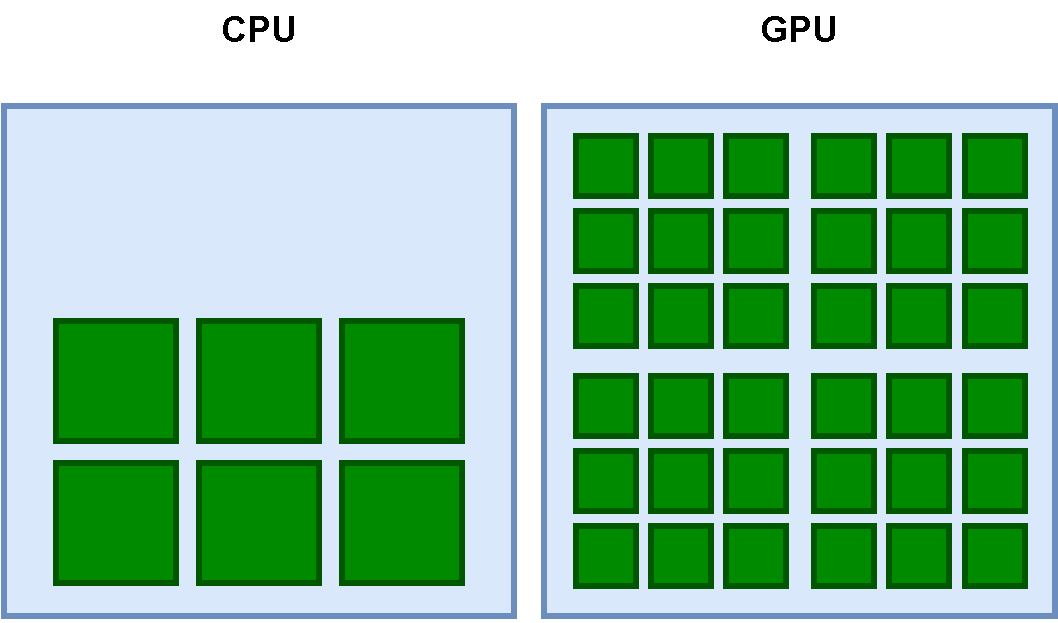
\includegraphics[width=8.0cm]{pictures/GPU_vs_CPU.pdf}
            \caption{Устройство CPU и GPU}
            \label{fig:cpuvsgpu}
        \end{figure}
    \end{minipage}\hfill
    \begin{minipage}[m]{0.4\linewidth}
        \begin{itemize}
            \item Если в CPU могут быть 2--16 ядер, то в GPU их сотни и тысячи
            \item Наличие нескольких ядер обеспечивает параллелизм и высокую эффективность обработки изображений
            \item OpenCL и Brahma.FSharp
        \end{itemize}
    \end{minipage}
\end{frame}

\end{document}